%<*probabil-2025-12-19-definicje-1>

Rozważmy sobie rozkład na \(\real^2\) o następujących własnościach:
\begin{itemize}
	\item gęstość wokół każdego punktu zależy jedynie od odległości od środka układu (w szczególności rotacja nie zmienia rozkładu).
	\item wartości współrzędnych \(x\) i \(y\) są od siebie niezależne.
	\item ten rozkład jest ciągły.
\end{itemize}

Okazuje się, że istnieje tylko jeden taki rozkład (z dokładnością do stałej), nazywamy go rozkładem normalnym. \\
%</probabil-2025-12-19-definicje-1>


\begin{definition}
	Definiujemy rozkład normalny (uogólniony) jako rozkład o następującej funkcji gęstości prawdopodobieństwa:

	\[ f_Z(z) =  \frac{1}{\sigma\sqrt{2\pi}}e^{-((z - \mu)/\sigma)^2/2} \]
\end{definition}

\begin{definition}
	Rozkład normalny o parametrach \(\mu\) i \(\sigma^2\) oznaczamy jako \(N(\mu , \sigma^2 )\).
\end{definition}

\begin{definition}
	Standardowy rozkład Normalny to rozkład normalny o parametrach \( \mu = 0\) i \( \sigma^2 = 1\); oznaczamy go (bez większego szoku) jako \(N(0, 1)\).
\end{definition}

%<*probabil-2025-12-19-definicje-2>
\begin{definition}
	Dystrybuantę standardowego rozkładu normalnego oznaczamy jako \( \Phi \), gdzie:
	\[
		\Phi = \frac{1}{\sqrt{2\pi}} \int_{\infty}^{z} e^{-\frac{t^2}{2}} \diff t
	\]
	Oraz:
	\[
		\Phi(-z) = 1 - \Phi(z)
	\]
	Ta całka generalnie nie jest do policzenia, jeżeli trzeba skorzystać z dystrybuanty to są do tego specjalne tabele wartości
\end{definition}

Funkcja gęstości prawdopodobieństwa standardowego rozkładu normalnego wygląda jak \sout{dzban} dzwon.

\begin{center}
	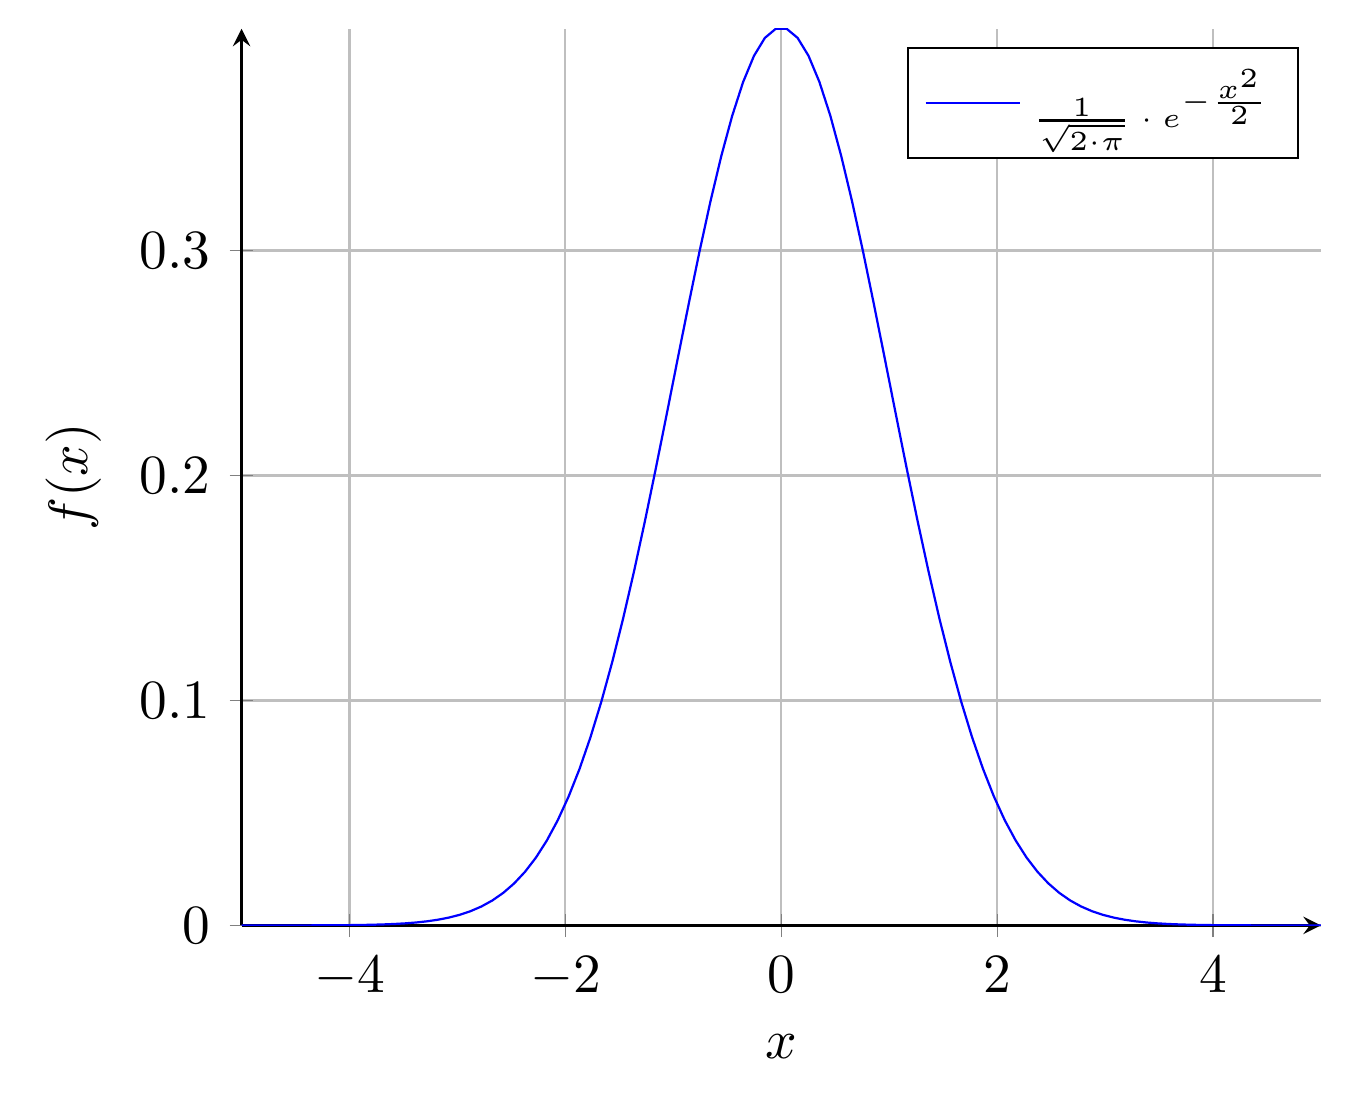
\begin{tikzpicture}[scale=2]
		\begin{axis}[
				axis lines = left,
				xlabel = \(x\),
				ylabel = {\(f(x)\)},
				ymajorgrids = true,
				xmajorgrids = true,
			]
			\addplot [
				domain=-5:5,
				samples=100,
				color=blue,
			]
			{(1/sqrt(2*pi)) * e^(-x^2/2)};
			\addlegendentry{\tiny \(\frac{1}{\sqrt{2 \cdot \pi}} \cdot e^{-\frac{x^2}{2}}\)}

		\end{axis}
	\end{tikzpicture}
\end{center}
%</probabil-2025-12-19-definicje-2>

